\chapter{Development of Smart-Doc System} 
\label{chap:ch4}

The previous chapter highlighted both the promise and the limitations of
AI-powered virtual patients: while feasible and increasingly sophisticated,
open questions remain regarding their capacity to foster complex reasoning,
support metacognition, and address cognitive biases in authentic learning
contexts. 

In response to these gaps, the \textbf{SmartDoc} platform was developed to
operationalize the theoretical and empirical foundations outlined in
Chapters~\ref{chap:ch2} and \ref{chap:ch3}. SmartDoc is designed as a
bias-aware clinical simulation environment that enables medical students to
practice diagnostic reasoning in natural language while receiving targeted
metacognitive feedback. The system integrates the principles of dual-process
reasoning, bias taxonomy, and debiasing strategies
(Chapter~\ref{chap:ch2}) with state-of-the-art advances in AI-powered virtual
patients (Chapter~\ref{chap:ch3}).

The architecture prioritizes three pedagogical goals:
\begin{enumerate}
    \item \textbf{Authenticity} — Realistic patient interactions through conversational interfaces that mimic real anamnesis, bridging the theory–practice gap.
    \item \textbf{Bias Awareness} — Detection of reasoning patterns associated with anchoring, confirmation, or premature closure, with just-in-time prompts to encourage reflection.
    \item \textbf{Structured Reflection} — Embedded checkpoints that support deliberate reflection and consolidation of diagnostic reasoning skills.
\end{enumerate}


In this chapter, we describe the design of the SmartDoc platform. Section~\ref{sec:system_design} introduces the conceptual system architecture and core components. Section~\ref{sec:llm_integration} explains how language models are integrated to balance realism and reliability. Section~\ref{sec:case_design_intent_driven} details the novel intent-driven case design, grounded in Mull et al.'s clinical case of cognitive error. Finally, Section~4.5 illustrates a typical workflow from the learner’s perspective.

\section{System Design} \label{sec:system_design}

\subsection{Conceptual Overview}

SmartDoc implements a modular simulation architecture built on the principle of \textit{progressive disclosure} (see Section~\ref{sec:debiasing}) and informed by experiential learning theory. The system separates responsibilities into three layers:
\begin{itemize}
    \item \textbf{Domain logic} — the reasoning engine and pedagogical rules,
    \item \textbf{API layer} — orchestrating communication and state management,
    \item \textbf{Presentation layer} — the learner-facing interface for interacting with the virtual patient.
\end{itemize}

\begin{figure}[h]
    \centering
    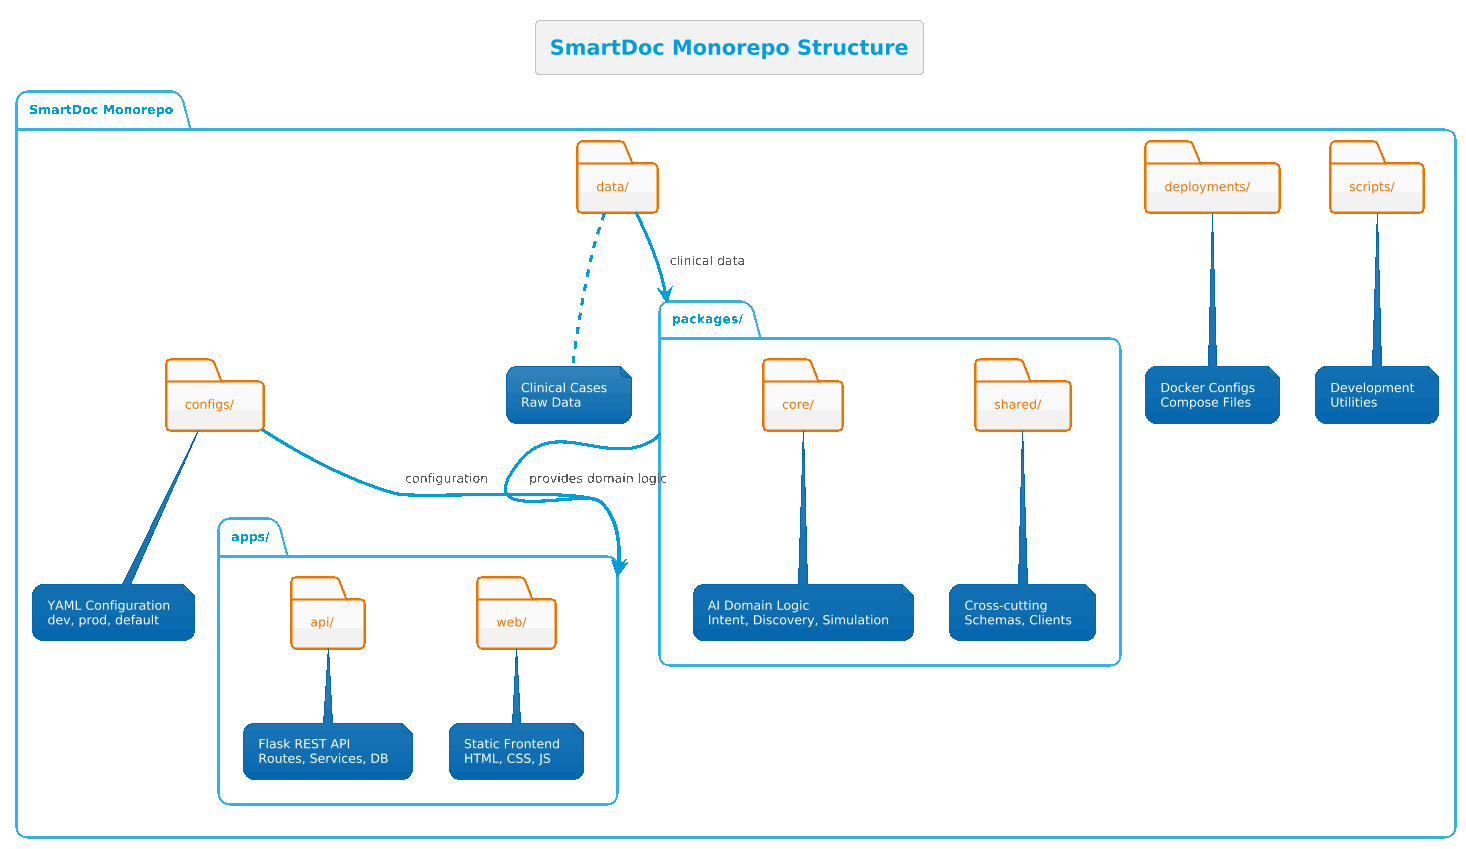
\includegraphics[width=0.86\textwidth]{figures/diagrams/high-level.png}
    \caption{High-level architecture of SmartDoc showing the interaction between core modules.}
    \label{fig:arch}
\end{figure}

At the core of the system lies the \textit{Intent-Driven Disclosure Manager}, which orchestrates three essential processes:
\begin{enumerate}
    \item \textbf{Understanding learner input} via an LLM-powered \emph{Intent Classifier},
    \item \textbf{Controlling information flow} through a \emph{Discovery Processor} that releases case data incrementally,
    \item \textbf{Monitoring reasoning patterns} through a \emph{Bias Analyzer} that detects bias-prone behaviors in real time.
\end{enumerate}

This architecture ensures that the simulation reflects authentic diagnostic practice (as emphasized in Chapter~\ref{chap:ch3}) while embedding cognitive safeguards to mitigate common reasoning errors (Chapter~\ref{chap:ch2}).

\subsection{Core Components}

\paragraph{Intent Classification.}
Learner utterances are mapped to a predefined set of diagnostic intents (e.g., request history, order test, suggest diagnosis). Rather than relying on rigid question trees, SmartDoc leverages natural language classification, allowing students to interact freely. This module operationalizes \textit{System~1 pattern recognition} while keeping pathways open for \textit{System~2 monitoring}.

\paragraph{Discovery Processing.}
Clinical information is released progressively, linked to learner queries. This implements the principle of \textbf{progressive disclosure}, ensuring that data emerges as a result of active inquiry rather than passive reception. Such design aligns with constructivist learning theory, promoting deep engagement over rote recall.

\paragraph{Simulation Engine.}
This orchestrates the entire learning loop:
\begin{quote}
\texttt{Student asks → Intent classified → Relevant information disclosed → Bias analysis applied → Response and feedback generated}
\end{quote}
It integrates reasoning traces with pedagogical scaffolds, ensuring each step is both educational and technically coherent.

\paragraph{Bias Analyzer.}
Bias detection is achieved through a combination of rule-based heuristics (e.g., repeated focus on one hypothesis) and LLM reasoning analysis. The module is directly grounded in the bias taxonomy (Section~\ref{sec:debiasing}), with real-time interventions such as:
\begin{quote}
\texttt{IF focus > 70\% on same hypothesis THEN prompt "What else could explain these findings?"}
\end{quote}
This transforms abstract debiasing strategies into actionable, in-the-moment coaching.

\paragraph{Session Management.}
All interactions are logged with bias timestamps and reflection responses. This provides a \emph{reasoning trace} for both formative feedback and summative assessment, enabling empirical evaluation of diagnostic reasoning skills (see Chapter~5).

\medskip
Together, these components implement a learning cycle where action, feedback, and reflection are tightly coupled, addressing the shortcomings of both traditional scripted simulations and unguided clinical encounters.

\section{Technical Implementation}
\label{sec:technical_implementation}

The SmartDoc system was implemented as a modular pipeline that translates free-text
learner inputs into pedagogically meaningful interactions. Its design reflects three
principles identified in earlier chapters: (i) \emph{progressive disclosure} of
clinical information (Chapter~\ref{chap:ch2}), (ii) \emph{real-time bias detection}
and metacognitive scaffolding (Chapter~\ref{chap:ch2}), and (iii) \emph{reliability
and reproducibility} across contexts, a key limitation noted in recent studies
(Chapter~\ref{chap:ch3}).

\subsection{Architecture \& Execution Pipeline}
\label{sec:execution_pipeline}

The pipeline follows a sequence of phases (Figure~\ref{fig:arch_pipeline}) that
mirror the reasoning process of a medical encounter. Each phase is encapsulated in
a dedicated module, enabling independent testing and future extension.

%\begin{figure}[h]
%    \centering
%    \includegraphics[width=0.85\textwidth]{figures/diagrams/pipeline.png}
%    \caption{Execution pipeline of SmartDoc showing modular processing stages.}
%    \label{fig:arch_pipeline}
%\end{figure}

\paragraph{1. Query Initiation and Routing.}
When a learner submits a question (e.g., \textit{``What are the patient’s vital
signs?''}), the system captures both the input and its context (session, diagnostic
phase). The request is passed to the central orchestrator, the
\textit{Intent-Driven Disclosure Manager}.

\paragraph{2. Intent Classification.}
The system determines what the learner is trying to do (e.g., gather history,
request labs, propose diagnosis). This operationalizes \textbf{System~1 pattern
recognition} while maintaining hooks for \textbf{System~2 monitoring}. If the
confidence of classification is low, the system applies fallbacks to preserve
robustness.

\paragraph{3. Discovery Processing.}
Once the intent is identified, the system decides what information to reveal.
Information is disclosed progressively, ensuring that students must \emph{seek}
evidence rather than receive it passively. This implements the pedagogical principle
of \emph{progressive disclosure}, encouraging active inquiry and preventing premature
closure.

\paragraph{4. Response Generation.}
Contextually appropriate responses are generated to maintain immersion:
\begin{itemize}
    \item anamnesis phase: family member dialogue,
    \item physical exam: descriptive findings,
    \item investigations: lab or imaging reports.
\end{itemize}
This provides authenticity while aligning with experiential learning theory.

\paragraph{5. Bias Detection and Session Logging.}
In parallel, the \emph{Bias Analyzer} monitors interaction patterns for signs of
anchoring, confirmation bias, or premature closure. Simple heuristics and LLM-based
analysis are combined, for example:

\begin{verbatim}
if focus_on_single_hypothesis > 70%:
    trigger_bias("anchoring")
    prompt_reflection("What else could explain these findings?")
\end{verbatim}

Detected events are logged with timestamps, creating a traceable record of reasoning
for both feedback and later research analysis.

\paragraph{6. Assembly and Delivery.}
The system compiles the patient reply, any new discoveries, bias warnings, and
progress indicators into a structured response. This is returned to the learner’s
interface and persisted for evaluation.

\medskip
This modular execution pipeline ensures controlled information flow (supporting
debiasing strategies), authentic immersion, and reproducibility—directly addressing
both pedagogical requirements and gaps identified in Chapter~\ref{chap:ch3}.

\subsection{LLM Integration}
\label{sec:llm_integration}

Given the variability of large language models, SmartDoc uses an abstraction
architecture to remain model-agnostic, ensuring both flexibility and reproducibility.

\subsubsection{Provider Abstraction}
All models are accessed through a standard \texttt{LLMProvider} interface with a
single \texttt{generate()} function. This design:
\begin{itemize}
    \item decouples pedagogical logic from vendor-specific implementations,
    \item allows deployment in diverse environments (local models for research,
    cloud-based models for production),
    \item supports substitution as models evolve, a key concern raised in the
    literature about sustainability.
\end{itemize}

\subsubsection{Dependency Injection}
Rather than hardcoding model use, providers are injected into each component
(e.g., intent classifier, bias analyzer). This enables:
\begin{itemize}
    \item isolated testing with mock providers,
    \item configuration tailored to educational scenarios (fast models for
    classification, more capable models for reasoning),
    \item consistent software engineering practices that ensure reliability.
\end{itemize}

\subsubsection{Prompt Engineering}
Prompts are modular and configurable, allowing experimentation without changing
the underlying code. Each prompt defines:
\begin{itemize}
    \item \emph{role}: e.g., “You are a patient describing symptoms,”
    \item \emph{context}: e.g., “current diagnostic phase = anamnesis,”
    \item \emph{constraints}: e.g., “reply in JSON format with labels.”
\end{itemize}
This structure supports A/B testing of pedagogical strategies (e.g., different
ways of framing reflection questions), linking directly to the literature’s call
for rigorous evaluation of design choices.

\subsubsection{Testing and Validation}
Robustness is ensured by simulating diverse model behaviours:
\begin{itemize}
    \item normal responses,
    \item timeouts or unavailable services,
    \item unexpected outputs.
\end{itemize}
Fallback mechanisms (e.g., switching to deterministic mappings) maintain
availability, ensuring that educational functionality is not compromised by
model instability. This directly addresses concerns in Chapter~\ref{chap:ch3}
regarding reproducibility of AI-VP systems.


\subsection{Database \& State Management}
\label{sec:db_state}

To support both responsive simulation and robust research analytics, SmartDoc
adopts a dual-layer state management architecture:
\begin{enumerate}
    \item \textbf{In-memory session state} --- ensures real-time responsiveness during the
    learner’s interaction with the virtual patient.
    \item \textbf{Persistent database storage} --- captures full reasoning traces,
    bias events, and reflection data for subsequent analysis.
\end{enumerate}
This separation allows the system to deliver immediate educational feedback while also
creating durable records for evaluation and research.

\subsubsection{Conceptual Schema}

The underlying schema is organized around \emph{educational workflows} rather than
technical implementation. Key entities include:

\begin{itemize}
    \item \texttt{Conversations}: the main unit of analysis, linking all messages and events.
    \item \texttt{Messages}: full history of learner queries and system responses.
    \item \texttt{DiscoveryEvents}: when and how clinical information was revealed
    (operationalizing \emph{progressive disclosure}).
    \item \texttt{BiasWarnings}: logged when patterns of anchoring, confirmation,
    or premature closure are detected (direct link to Chapter~\ref{chap:ch2}).
    \item \texttt{ReflectionResponses}: learner’s answers to structured prompts,
    supporting deliberate reflection research.
    \item \texttt{DiagnosisSubmissions}: final diagnostic hypotheses with
    justification, enabling outcome evaluation.
\end{itemize}

A simplified view of the schema is illustrated in
Figure~\ref{fig:db_schema}. This design ensures that each learner
session produces a rich, analyzable dataset that links behaviour
(intents, queries) with outcomes (diagnosis accuracy, bias awareness).

\begin{figure}[h]
    \centering
    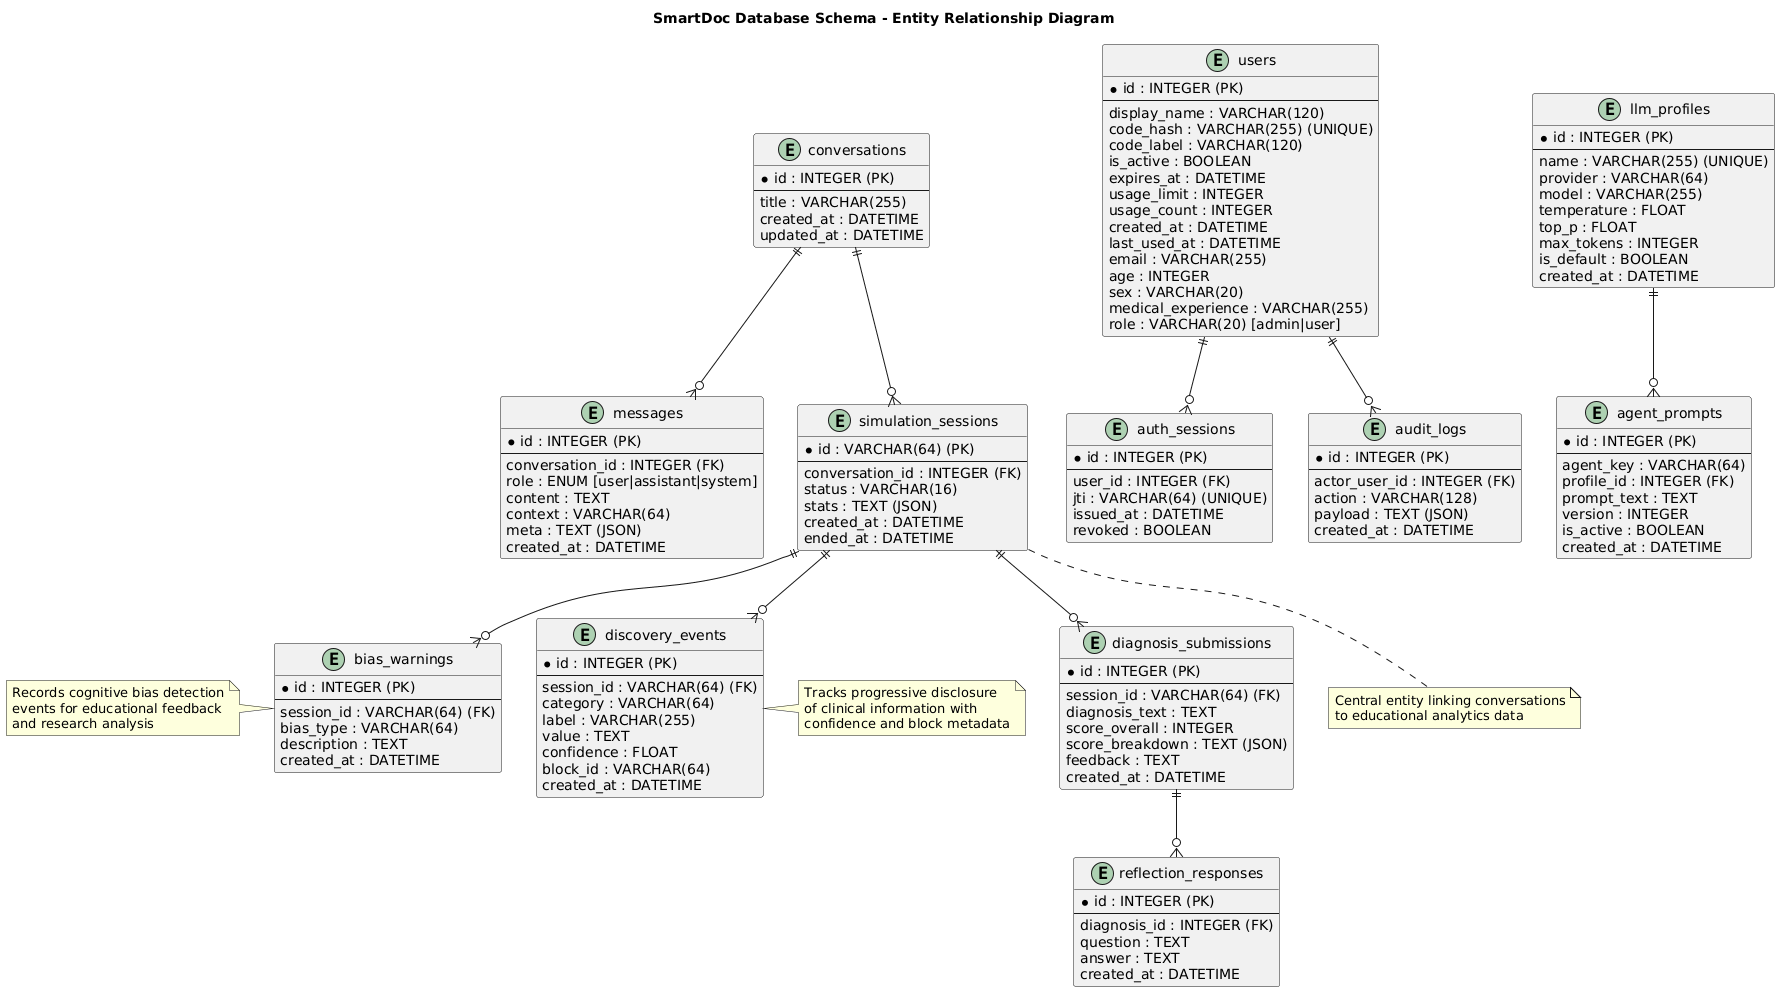
\includegraphics[width=0.8\textwidth]{figures/diagrams/erdb.png}
    \caption{Conceptual schema: capturing reasoning traces, bias events, and reflection data.}
    \label{fig:db_schema}
\end{figure}

\subsubsection{State Management Architecture}

During a simulation, the \emph{Progressive Disclosure Store} maintains
session-level state in memory (revealed information blocks, queries,
working hypotheses). Hooks such as \texttt{on\_reveal} or
\texttt{on\_interaction} trigger updates to the database when key
pedagogical events occur. This allows the system to both:
\begin{itemize}
    \item deliver instant responses to the learner, and
    \item log structured traces for later analysis.
\end{itemize}

Pseudo-code sketch:

\begin{verbatim}
on_reveal(info_block):
    update_session_state(info_block)
    log_to_database(event="discovery", timestamp=now)

on_bias_detected(bias_type):
    issue_warning(bias_type)
    log_to_database(event="bias", bias=bias_type, timestamp=now)
\end{verbatim}

This event-driven design ensures that cognitive bias detection (Chapter~\ref{chap:ch2})
and reflection prompts are not only experienced by the learner but also captured for
empirical study (Chapter~\ref{chap:ch3}).

\subsubsection{Choice of Database Technology}

For research purposes, portability and reproducibility were prioritised.
A lightweight single-file database (\emph{SQLite}) was chosen because it:
\begin{itemize}
    \item allows easy sharing of complete simulation datasets for replication studies,
    \item eliminates external dependencies for participants in multi-site trials,
    \item guarantees data integrity even in abrupt session terminations.
\end{itemize}
Although SQLite does not support massive concurrency, SmartDoc’s use case involves
individual or small-cohort learning sessions, making this a pragmatic and effective choice.
The abstraction layer (SQLAlchemy) ensures that the system can migrate to enterprise-grade
databases (e.g. PostgreSQL) if future large-scale deployments require it.

\subsubsection{Logging and Reproducibility}

SmartDoc implements structured logging for both technical and pedagogical events.
For each session, the following are captured:
\begin{itemize}
    \item learner queries and classified intents,
    \item information blocks revealed and their sequence,
    \item bias warnings triggered,
    \item reflection responses submitted.
\end{itemize}

These logs create a complete \emph{reasoning trace}, enabling:
\begin{enumerate}
    \item \textbf{Formative feedback} --- personalised debriefs for learners.
    \item \textbf{Summative evaluation} --- assessment of diagnostic accuracy and
    bias awareness.
    \item \textbf{Research analytics} --- large-scale studies of interaction patterns,
    replicating the calls in Chapter~\ref{chap:ch3} for more transparent evaluation
    of AI-VPs.
\end{enumerate}
By embedding reproducibility at the data layer, SmartDoc ensures that each learning
session doubles as a research opportunity.

\subsection{Deployment}
\label{sec:deployment}

A critical requirement for SmartDoc is that it can be reliably deployed in both
research and educational settings. The deployment architecture was therefore designed
with three guiding principles:

\begin{enumerate}
    \item \textbf{Reproducibility} — ensuring that the same configuration can be
    reproduced across different sites and machines.
    \item \textbf{Scalability} — enabling the platform to support cohorts of learners
    by scaling up model inference capacity when needed.
    \item \textbf{Accessibility} — minimizing technical barriers for institutions,
    favouring lightweight setups that do not require specialised infrastructure.
\end{enumerate}

\subsubsection{Containerisation and Reproducibility}

To guarantee consistent behaviour across environments, the system is distributed as
containerised services (e.g., backend API, database, language model interface).
This encapsulation ensures that all dependencies are versioned and portable, allowing
educational institutions or research collaborators to reproduce experiments without
lengthy installation steps. Containerisation also aligns with recent calls in the
literature for reproducible AI-based educational systems (see Chapter~\ref{chap:ch3}).

\subsubsection{Model Hosting and Flexibility}

SmartDoc supports two main deployment modes:
\begin{itemize}
    \item \emph{Local hosting}, using lightweight models for research replication
    and settings with limited internet access.
    \item \emph{Cloud hosting}, connecting to high-accuracy commercial models for
    large-scale or production use.
\end{itemize}

This dual-mode design reflects a balance between \emph{cost}, \emph{accuracy}, and
\emph{data governance}, allowing institutions to select the configuration best suited
to their pedagogical and ethical context.

\subsubsection{Scalability Considerations}

Although individual learners typically interact with the system in isolation,
classroom or multi-cohort settings require concurrent sessions. The architecture
therefore supports horizontal scaling: additional inference services can be launched
in parallel, each serving multiple SmartDoc instances. This ensures that response
times remain low, preserving immersion and educational value even with larger groups.

\subsubsection{Security and Data Integrity}

Given that learner interactions include reasoning traces and reflection data,
deployment must also ensure \emph{data integrity and privacy}. The platform
implements:
\begin{itemize}
    \item role-based access (distinguishing learners, educators, administrators),
    \item encrypted storage of sensitive configuration parameters,
    \item automated backups of educational data.
\end{itemize}

These safeguards align with ethical considerations around learner data use raised
in Chapter~\ref{chap:ch3}.

\subsubsection{Educational Impact of Deployment Design}

By prioritising reproducibility and portability, SmartDoc enables institutions
to adopt the platform with minimal setup, making bias-aware simulation accessible
beyond well-resourced centres. The scalability features ensure that the system
remains responsive in group teaching contexts, while the emphasis on security
reinforces trust in its use for formal training. Together, these choices demonstrate
that deployment is not only a technical concern but also an \emph{educational enabler},
supporting widespread adoption and rigorous evaluation.

\subsection{User Interfaces}
\label{sec:user_interfaces}

The SmartDoc platform provides a web-based interface designed explicitly for
clinical education. Its design prioritises usability, immersion, and alignment
with pedagogical principles such as progressive disclosure, scaffolded learning,
and metacognitive reflection.

\subsubsection{Interface Architecture}

Three complementary interfaces support different roles:

\begin{itemize}
    \item \textbf{Simulation Interface} — the learner-facing environment for
    conducting clinical interviews and reasoning through cases.
    \item \textbf{Administrative Dashboard} — tools for educators and researchers
    to configure cases, manage learners, and monitor outcomes.
    \item \textbf{Authentication Portal} — secure entry point with role-based
    access for learners and instructors.
\end{itemize}

This separation of concerns reflects the dual needs of \emph{educational delivery}
and \emph{research oversight}.

\subsubsection{Medical Simulation Interface}

The simulation interface is organised around the phases of diagnostic reasoning,
each represented as a tab or section (see Figure~\ref{fig:ui_wireframe}):

\begin{enumerate}
    \item \textbf{Patient Information} — static demographic and background data.
    \item \textbf{Clinical Interview (Anamnesis)} — free-text dialogue with the
    virtual patient or family member.
    \item \textbf{Physical Examination} — simulated physical findings provided
    upon request.
    \item \textbf{Investigations} — laboratory and imaging results, revealed
    progressively.
    \item \textbf{Results \& Reflection} — final diagnosis entry, performance
    summary, and metacognitive checkpoint.
\end{enumerate}

\begin{figure}[h]
    \centering
    \includegraphics[width=0.8\textwidth]{figures/diagrams/ui-wireframe.png}
    \caption{Wireframe of the learner-facing interface. Tabs reflect the phases of
    diagnostic reasoning, supporting progressive disclosure.}
    \label{fig:ui_wireframe}
\end{figure}

This phased design implements \emph{progressive disclosure}, requiring learners
to actively request information rather than passively receiving it. It mirrors the
iterative nature of real diagnostic encounters.

\subsubsection{Bias Awareness and Reflection Prompts}

Two features embed the debiasing strategies discussed in
Chapter~\ref{chap:ch2}:

\begin{itemize}
    \item \textbf{Bias Warnings} — triggered when the Bias Analyzer detects
    patterns of anchoring, confirmation, or premature closure. Warnings are
    displayed non-intrusively, e.g., \textit{``You seem focused on a single
    hypothesis. Consider alternative explanations.''}
    \item \textbf{Metacognitive Checkpoints} — at key points (e.g., before
    finalising a diagnosis), learners must reflect on their reasoning:
    \begin{verbatim}
    - What evidence supports your current diagnosis?
    - What evidence contradicts it?
    - What alternative diagnoses should be considered?
    \end{verbatim}
\end{itemize}

These features operationalise \emph{cognitive forcing strategies} and
\emph{deliberate reflection}, turning abstract debiasing methods into
practical, in-the-moment educational interventions.

\subsubsection{Administrative Dashboard}

The educator-facing dashboard provides case configuration and oversight tools.
Key functions include:
\begin{itemize}
    \item adding or modifying cases and bias triggers,
    \item managing cohorts of learners,
    \item reviewing aggregated analytics (bias frequency, diagnostic accuracy,
    reflection quality).
\end{itemize}

This supports both curriculum integration and educational research, enabling
instructors to monitor not only outcomes but also \emph{processes of reasoning}.

\subsubsection{Educational Design Principles}

The UI design is grounded in the following principles:

\begin{itemize}
    \item \textbf{Cognitive load management} — phased workflows prevent
    overwhelming learners with information.
    \item \textbf{Immediate feedback} — bias warnings appear in real time,
    guiding learners without derailing immersion.
    \item \textbf{Scaffolded reflection} — structured prompts encourage deliberate
    reflection at moments of diagnostic closure.
    \item \textbf{Traceability} — interaction histories are logged, creating
    reasoning traces for personalised feedback and research.
\end{itemize}

\medskip
Together, these interface elements embody the alignment between technology and
pedagogy: SmartDoc is not only a functional application, but an
\emph{educational instrument} deliberately crafted to foster bias awareness,
metacognition, and diagnostic expertise.

\subsection{Case Design: Intent-Driven Simulation}
\label{sec:case_design_intent_driven}

The SmartDoc platform introduces a novel approach to clinical case design that embeds
educational triggers and bias detection directly into the case structure itself. This
intent-driven simulation model represents a significant innovation in medical education
technology, moving beyond traditional linear case presentations to create dynamic,
conversational learning experiences.

\subsubsection{Case Schema Architecture}

Each SmartDoc case is defined using a structured schema that integrates
\textbf{progressive disclosure}, \textbf{bias triggers}, and \textbf{reflection notes}
directly into the case content. This ensures that diagnostic reasoning, bias
awareness, and metacognition are not peripheral features but are embedded in the
simulation itself.

A minimal case definition includes four core elements:

\begin{enumerate}
    \item \textbf{Initial Presentation} — chief complaint and basic context.
    \item \textbf{Information Blocks} — modular clinical facts (history, exam,
    labs, imaging, medications), progressively revealed through learner queries.
    \item \textbf{Bias Triggers} — metadata that defines when and how anchoring,
    confirmation, or framing biases are likely to occur, along with corrective prompts.
    \item \textbf{Educational Notes} — learning objectives, clinical pearls, and
    structured reflection questions linked to the case.
\end{enumerate}

\begin{lstlisting}[language=json]
{
  "caseId": "mull_case",
  "caseTitle": "An elderly woman with 'heart failure'",
  "initialPresentation": {
    "chiefComplaint": "Worsening shortness of breath",
    "historyOfPresentIllness": "Elderly Spanish-speaking woman, history provided by son..."
  },
  "informationBlocks": [...],
  "biasTriggers": {...},
  "educationalNotes": {...}
}
\end{lstlisting}

By embedding these components into a single schema, SmartDoc avoids the limitations of
scripted, branching cases. Instead, the case itself defines when information is revealed,
where bias prompts are activated, and how reflection is scaffolded. This modular structure
serves as the foundation for the progressive disclosure and bias-aware design principles
described in the following sections.


\subsubsection{Information Blocks and Progressive Disclosure}

Information is stored in modular \emph{information blocks}, each annotated with:
\begin{itemize}
    \item \textbf{level} — depth of inquiry required (e.g., Level 1 = basic, Level 2 = deeper follow-up),
    \item \textbf{reveal policy} — when the block is disclosed (\texttt{immediate}, \texttt{escalate}, \texttt{conditional}),
    \item \textbf{prerequisites} — other blocks that must be revealed first,
    \item \textbf{isCritical} — whether the block is essential to reach the correct diagnosis.
\end{itemize}

\paragraph{Example block.}
\begin{lstlisting}[language=json]
{
  "blockId": "critical_infliximab",
  "blockType": "Medications",
  "content": "Records reveal the patient has been receiving infliximab for rheumatoid arthritis.",
  "isCritical": true,
  "intentTriggers": ["meds_full_reconciliation_query"],
  "level": 2,
  "prerequisites": ["meds_ra_uncertainty"],
  "revealPolicy": "escalate"
}
\end{lstlisting}

In this example, the infliximab clue (key to diagnosing tuberculosis) is only revealed
after learners probe medication history in detail — resisting \emph{premature closure}.
This mirrors real-world reasoning and forces learners to engage in deeper inquiry.

\paragraph{Progressive disclosure in practice.}
\begin{itemize}
    \item \textbf{Level 1:} basic data (vital signs, initial medication list) disclosed immediately.
    \item \textbf{Level 1 (uncertainty):} queries about rheumatoid arthritis drugs return
    only partial information, requiring persistence.
    \item \textbf{Level 2 (critical):} infliximab use is revealed only after escalation or
    prerequisite discovery.
\end{itemize}

\begin{figure}[h]
    \centering
    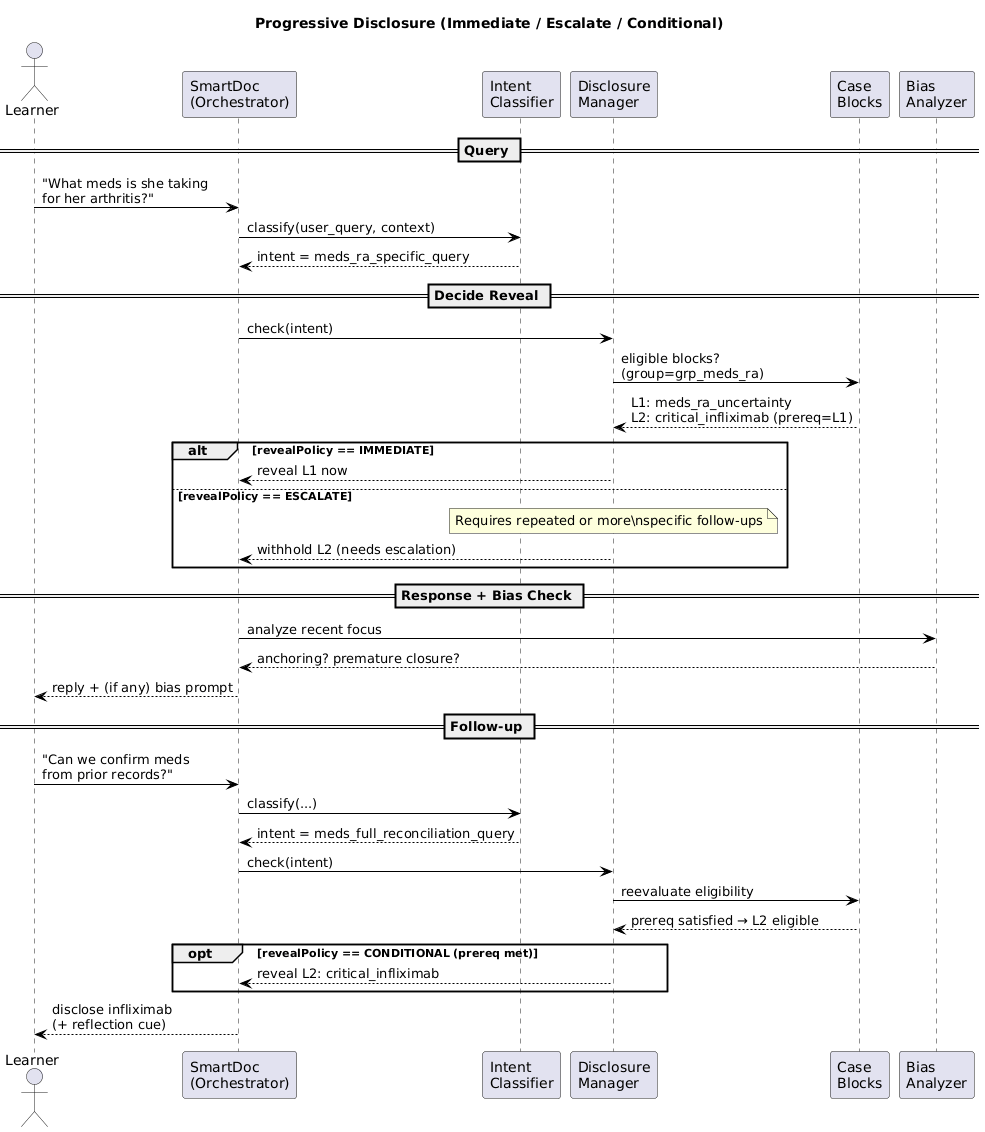
\includegraphics[width=0.85\textwidth]{figures/diagrams/progressive-disclosure.png}
    \caption{Progressive disclosure ladder: Level 1 = surface data; Level 2+ = deeper
    information, often bias-resistant and critical for correct diagnosis.}
    \label{fig:progressive_disclosure}
\end{figure}

\paragraph{Educational link.}
This mechanism operationalises:
\begin{itemize}
    \item \textbf{Anchoring bias} — learners who stop at the BNP or first chest X-ray
    risk missing contradictory findings.
    \item \textbf{Premature closure} — learners who fail to escalate queries miss the
    infliximab clue.
    \item \textbf{Framing bias} — the initial “elderly woman with heart failure” label
    influences which blocks are pursued.
\end{itemize}

\subsubsection{Embedded Bias Triggers}

Bias triggers are encoded directly in case metadata, allowing real-time monitoring of
learner reasoning. Example (anchoring):

\begin{lstlisting}[language=json]
"biasTriggers": {
  "anchoring": {
    "anchorInfoId": "imaging_cxr_preliminary",
    "contradictoryInfoId": "critical_echo",
    "description": "Anchoring on preliminary CXR delays recognition of normal echo."
  }
}
\end{lstlisting}

\paragraph{Pseudo-code for bias detection.}
\begin{verbatim}
IF recent queries focus >70% on "heart/cardiac":
    Trigger("Anchoring Bias Warning")
    Prompt("What else could explain dyspnoea?")
\end{verbatim}

This transforms abstract debiasing strategies (e.g., cognitive forcing) into concrete,
in-the-moment interventions.

\subsubsection{Educational Notes and Reflection Support}

Each case embeds learning objectives, clinical pearls, and reflection prompts. Example:

\begin{lstlisting}[language=json]
"educationalNotes": {
  "learningPoints": ["Medication reconciliation is crucial in multimorbidity"],
  "clinicalPearls": ["TNF-alpha inhibitors like infliximab increase TB risk"],
  "biasAwareness": ["Anchoring on initial impressions delays correct diagnosis"]
}
\end{lstlisting}

At diagnostic closure, structured prompts require learners to reflect:
\begin{verbatim}
- What evidence supports your diagnosis?
- What evidence contradicts it?
- What alternative explanations remain plausible?
\end{verbatim}

This operationalises \textbf{deliberate reflection} (Chapter~\ref{chap:ch2}) and ensures
that reflection is not optional but embedded in the workflow.

\subsubsection{Application: The Mull Case}

The prototype case adapts Mull et al.~\parencite{mull_cognitive_2015}, in which an
elderly woman with dyspnoea was repeatedly misdiagnosed with heart failure due to
anchoring, confirmation, and framing biases. SmartDoc encodes this case by:
\begin{itemize}
    \item framing the presentation as “elderly patient with heart failure”,
    \item embedding anchoring triggers around chest X-ray and BNP results,
    \item requiring detailed medication reconciliation to reveal infliximab use.
\end{itemize}

\subsubsection{Educational Impact and Innovation Summary}

The intent-driven design provides several innovations:

\begin{enumerate}
  \item \textbf{Conversational learning} — natural dialogue replaces scripted question trees.
  \item \textbf{Embedded bias education} — bias triggers built into case metadata.
  \item \textbf{Progressive disclosure} — learners earn critical clues by resisting bias-prone shortcuts.
  \item \textbf{Scaffolded reflection} — structured checkpoints operationalise metacognition.
  \item \textbf{Research-ready design} — interaction logs capture reasoning traces for analysis.
\end{enumerate}

In this way, SmartDoc transforms case-based learning from passive fact recall to active,
bias-aware clinical reasoning practice.

\subsection{Example Workflow}

\textbf{TODO}

\section{Summary}
\label{sec:summary}

This chapter described the development of SmartDoc, highlighting how technical
decisions were guided by pedagogical principles and empirical evidence. The
platform was designed not merely as a simulation engine, but as a bias-aware
educational tool aligned with the theoretical foundations of dual-process
reasoning, cognitive bias taxonomy, and deliberate reflection (Chapter~\ref{chap:ch2}),
and addressing limitations identified in the literature on AI-powered virtual
patients (Chapter~\ref{chap:ch3}).

\subsection{Key Design Principles}

Three principles informed the system architecture:

\begin{enumerate}
    \item \textbf{Progressive Disclosure} --- ensuring learners actively
    request information, reducing premature closure and supporting authentic
    reasoning.
    \item \textbf{Bias-Aware Design} --- embedding triggers for anchoring,
    confirmation, and framing biases directly in case metadata, allowing
    real-time monitoring and corrective prompts.
    \item \textbf{Metacognitive Scaffolding} --- integrating reflection
    checkpoints and educational notes to foster deliberate reflection on
    diagnostic reasoning.
\end{enumerate}

\subsection{Core Technical Contributions}

SmartDoc advances the state of AI-powered simulation through:

\begin{itemize}
    \item an intent-driven disclosure engine that supports natural
    conversational learning rather than scripted branching,
    \item a bias analyzer that transforms cognitive forcing strategies into
    just-in-time prompts,
    \item a case schema that unifies clinical content with educational metadata,
    enabling both learner guidance and research analytics.
\end{itemize}

Together, these contributions address two persistent gaps: (i) the lack of
simulation systems that make reasoning \emph{visible and improvable}, and (ii)
the need for reproducibility and transparency in AI-based educational tools.

\subsection{Experimental Configuration}

While SmartDoc is capable of providing \emph{live bias feedback} during learner
interactions, this feature was intentionally disabled in the evaluation study
with clinical apprentices (see Chapter~\ref{chap:results}). Instead,
participants completed the interview without intervention and only after
submitting a final diagnosis were they presented with structured reflection
prompts and LLM-generated feedback on:
\begin{itemize}
    \item diagnostic accuracy,
    \item relevant learning points,
    \item possible biases exhibited,
    \item and mitigation strategies for future reasoning.
\end{itemize}

This configuration ensured that learners’ reasoning processes were not
artificially altered during the simulation, while still allowing SmartDoc to
capture bias-prone behaviours for later analysis.

\subsection{From Design to Evaluation}

By embedding theory-driven design into a robust technical framework, SmartDoc
demonstrates how cognitive psychology, bias taxonomy, and simulation principles
can be operationalised in an AI-powered educational system. The platform
introduces several innovations: intent-driven case design, embedded bias
triggers, and structured reflection checkpoints, all aimed at making clinical
reasoning both visible and improvable.

Having established the rationale and technical architecture of SmartDoc, the
next chapter evaluates how these design decisions perform in practice.
Chapter~\ref{chap:results} presents the results of pilot testing with clinical
interns, examining the system’s usability, realism, and educational impact, and
assessing whether SmartDoc can effectively raise learners’ awareness of cognitive
bias in diagnostic reasoning.


